%NOTE(@SomeoneSerge): copy-pasted as is from private notes, may diverge from the upstream version.

\documentclass{beamer}

\usepackage{minted}
\usepackage{xeCJK}
\usepackage{fontspec}
\setmainfont[
  Ligatures=TeX,
  Extension=.otf,
  BoldFont=cmunbx,
  ItalicFont=cmunti,
  BoldItalicFont=cmunbi,
]{cmunrm}

\setmonofont{Source Code Pro Medium}
% \setmonofont{CMU Typewriter Text} % Original used in Berlin

\usepackage{fontawesome5}
\usepackage{hyperref}
\usepackage{url}

\usepackage{tikz}
\usetikzlibrary{positioning,matrix,fit}
\usepackage{forest}
\useforestlibrary{linguistics}

\usepackage{newunicodechar}
\newunicodechar{❌}{\faCheck}

\title{Evanix: Scheduling as (M)ILP}
\subtitle{GSoC'24}
\author{@sinanmohd and @SomeoneSerge}
% \institute{Overleaf}
\date{2024}

\begin{document}

\frame{\titlepage}

\begin{frame}
\frametitle{What: ``build budgets''}
\resizebox{0.60\textwidth}{!}{
\begin{forest}
every tree node/.style={align=center,anchor=north},
drvbuild/.style={circle, draw=red!60, fill=red!5, very thick, minimum size=10mm},
drvsubst/.style={circle, draw=yellow!60, fill=yellow!5, very thick, minimum size=10mm},
drvready/.style={circle, draw=green!60, fill=green!5, very thick, minimum size=10mm},
triangle/.style={regular polygon, regular polygon sides=3},
subtreeready/.style={triangle, draw=green!60, fill=green!5, very thick, minimum size=10mm},
subtreebuild/.style={triangle, draw=red!60, fill=red!5, very thick, minimum size=10mm},
bigger/.style={minimum size=20mm},
[,phantom
    [a,drvbuild
        [torch, name=torch, drvsubst]
        [opencv,drvready
            [[[[..., name=aClosure, subtreeready, bigger
                [,phantom]
                [glibc, drvready]]]]]
        ]
    ]
    [a-cuda,drvbuild
        [torch-cuda, drvbuild
            [, phantom]
            [nccl, drvbuild
                [, phantom]
                [..., name=aCudaClosure, subtreebuild]
            ]
        ]
        [opencv-cuda, name=opencv-cuda, drvbuild]
    ]
]
\draw[->] (aCudaClosure) -- (aClosure);
\draw[->] (opencv-cuda) -- (aCudaClosure);
\draw[->] (torch) -- (aClosure);
\end{forest}
}
\end{frame}

\begin{frame}[fragile]
\frametitle{Why: short circuiting}
\begin{itemize}
\item Run \verb|nix-build| in github actions
\item Bump pinned \verb|nixpkgs|
\item See the action time out on a mass rebuild
\item Smart solution: \verb|¯\_(ツ)_/¯|
\item Low-tech hack: tell Nix to choose \(\leq 100\) derivations to build
\end{itemize}
\end{frame}

\begin{frame}
\frametitle{How: Integer Linear Programming}
\begin{itemize}
\item Derivations: \( 1, \ldots, n \).
\item User asked for derivation \( i \)? \( v=(v_1, \ldots, v_n)\in\{0,1\}^n \).
\item Would we have to build it? \( c=(c_1, \ldots, c_n)\in\{0,1\}^n \).
\item Do we choose to ``realize'' it? \( x=(x_1, \ldots, x_n)\in\{0,1\}^n \).
\item ``Value'' of the plan: \( \langle x, v \rangle. \)
\item Maximum \(\sharp\) builds: \( \langle x, c \rangle \leq C. \)
\item Derivation \( i \) depends on \( j \): \( x_i \leq x_j \).
\end{itemize}
\end{frame}

\begin{frame}[fragile]
\frametitle{Demo: PoC in C using HIGHS}
\begin{minted}[fontsize=\tiny]{console}
$ evanix --dry-run --flake .#packages.x86_64-linux --max-builds 4 --solver-report
...
❌ refusing to build /nix/store/...-llama-cpp-cuda-0.0.0.drv, cost: 9
❌ refusing to build /nix/store/...-python3.12-llama-scripts-0.0.0.drv, cost: 2
❌ refusing to build /nix/store/...-llama-cpp-x86_64-w64-mingw32-0.0.0.drv, cost: 22
🛠️ nix-build --out-link result-default /nix/store/...-llama-cpp-blas-0.0.0.drv
🛠️ nix-build --out-link result-mpi-cpu /nix/store/...-llama-cpp-blas-mpi-0.0.0.drv
🛠️ nix-build --out-link result-rocm /nix/store/...-llama-cpp-rocm-0.0.0.drv
🛠️ nix-build --out-link result-vulkan /nix/store/...-llama-cpp-vulkan-0.0.0.drv
\end{minted}

@sinanmohd
\end{frame}

\begin{frame}[fragile]
\frametitle{Integration Tests (tvix would've solved this?)}
\begin{minted}[fontsize=\tiny]{nix}
{
  imports = [
    {
      dag.nodes.a.cache = "remote";
      dag.nodes.b.cache = "remote";
      dag.nodes.d.goal = true;
      dag.test.unconstrained.builds = 2;
      dag.test.unconstrained.downloads = 2;
    }
  ];
    nodes =
      {
        a = goalDependsOn [ "u" "v" ];
        b = goalDependsOn [ "u" "v" ];
        c = goalDependsOn [ "u" "v" ];
        d = goalDependsOn [ "w" ];
        u = { };
        v = { };
        w = { };
      };
};
\end{minted}

\end{frame}

\begin{frame}
\frametitle{Different costs}

\begin{itemize}
\item Old: \( c\in\{0,1\}^n \).
\item Might as well: \( c\in\mathbb{R}^n \).
\item Might as well: \( c_i = \text{estimated build time of}~i \).
\end{itemize}
\end{frame}

\begin{frame}[fragile]
\frametitle{Different costs: how}

\begin{itemize}
\item \verb|inputDrvs| \(=~\{\ldots,\textrm{/nix/store/...-cmake-3.29.6.drv}, \ldots\}\)
\item Mask hash and version
\item Training: each \verb|build_id| in NixOS Hydra is a row; regress \verb|stoptime - starttime|; prune
\item Inference: scan new drv, filter \verb|pname|s, set \(1\)s, multiply \& add
\end{itemize}
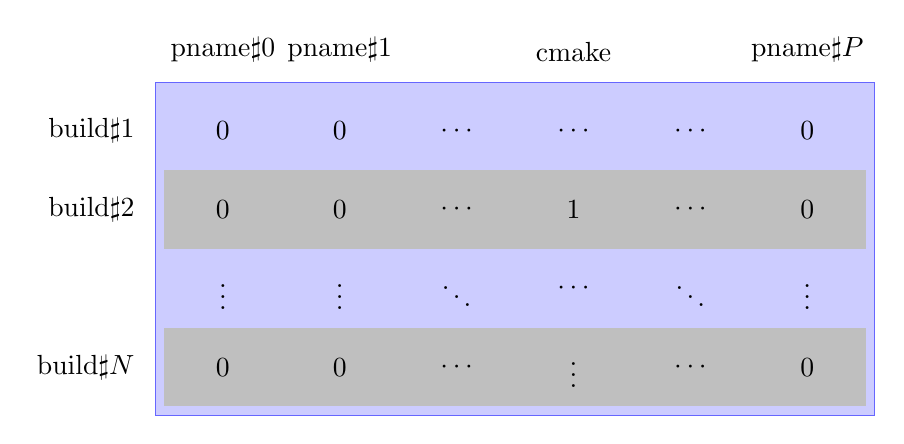
\begin{tikzpicture}
  \node [
    matrix of nodes, nodes in empty cells,
    nodes={text width=1.25cm, align=center, minimum height=1.25em, anchor=center},
    every even row/.style={nodes={fill=gray!50}},
    fill=blue!20,draw=blue!60,nodes={fill=blue!20,minimum size=10mm},
    ] (mymtrx) {
    \node [name=r1] {0}; & \node[name=c2]{0};      & \node{\(\cdots\)}; & \node[name=colNvcc]{\(\cdots\)}; & \node{\(\cdots\)};  & \node [name=collast]{0}; \\
    \node [name=rllama] {0}; & \node{0};  & \node{\(\cdots\)}; & \node{\(1\)}; & \node{\(\cdots\)};  & \node {0}; \\
    \node {\(\vdots\)};  & \node{\(\vdots\)}; & \node{\(\ddots\)}; & \node{\(\cdots\)}; & \node {\(\ddots\)}; & \node {\(\vdots\)}; \\
    \node [name=rlast] {0}; & \node{0};       & \node{\(\cdots\)}; & \node{\(\vdots\)}; & \node{\(\cdots\)}; & \node {0}; \\
  };
  \node[left=0.25cm of r1]{build\(\sharp 1\)};
  \node[left=0.25cm of rllama]{build\(\sharp 2\)};
  \node[left=0.25cm of rlast]{build\(\sharp N\)};
  \node[above=0.25cm of collast]{pname\(\sharp P\)};
  \node[above=0.25cm of r1]{pname\(\sharp 0\)};
  \node[above=0.25cm of c2]{pname\(\sharp 1\)};
  \node[above=0.25cm of colNvcc]{cmake};
\end{tikzpicture}
\end{frame}

\begin{frame}
\frametitle{Anything left to do? Can we do better?}
A ton
\end{frame}
\end{document}
